% ==============================================================================
% SECCIÓN DE COMPLEJIDAD Y RESULTADOS DEL SOLVER (FORMATO IEEEtran)
% ==============================================================================

\section{An\'alisis de Complejidad y Evaluaci\'on Experimental del Solver}
\label{sec:complexity_and_experiments}

\subsection{Complejidad Te\'orica vs. Espacio de B\'usqueda Podado}
El espacio de b\'usqueda bruto (no restringido) de una cuadr\'{\i}cula KenKen de orden $n$ escala seg\'un:
\begin{equation}
    |\mathcal{S}_{\text{bruto}}| = n^{n^2} = \mathcal{O}(n^{n^2})
\end{equation}
Para $n=3$, $|\mathcal{S}| = 3^9 = 19{,}683$. Para $n=9$, el espacio combinatorial alcanza $9^{81} \approx 1.96 \times 10^{77}$ estados factibles brutos, una cifra comparable al n\'umero total de \'atomos estimados en el universo observable.

Al imponer la restricci\'on global de no repetici\'on por filas (\ref{eq:alldiff_row}), cada l\'{\i}nea ortogonal se restringe a las $n!$ permutaciones del conjunto $\{1, \dots, n\}$, contrayendo el espacio a:
\begin{equation}
    |\mathcal{S}_{\text{filas}}| = (n!)^n
\end{equation}
Para $n=9$, $(9!)^9 \approx 1.09 \times 10^{50}$ estados. La adici\'on de las restricciones de columna reduce a\'un m\'as el espacio factible al conjunto de Cuadrados Latinos $L(n)$, acotado asint\'oticamente por $(n!)^{2n} / n^{n^2}$. Finalmente, la conjunci\'on de las jaulas aritm\'eticas reduce el espacio a una soluci\'on \'unica (en problemas bien formulados).

En la pr\'actica, el solucionador CP-SAT~\cite{perron2023cpsat, perron2024ortools} integra la tecnolog\'{\i}a de \textit{Lazy Clause Generation} (LCG)~\cite{ohrimenko2009lazy}, que mapea dominios y cotas lineales en cl\'ausulas booleanas aprendidas durante el filtrado. Esto permite que la propagaci\'on deduzca las asignaciones factibles en el \textbf{nodo ra\'{\i}z}, eliminando por completo la necesidad de b\'usqueda con retroceso (\textit{backtracking}).

\subsection{Resultados Experimentales del Benchmark CP-SAT \texorpdfstring{($n=3$ a $n=9$)}{(n=3 a n=9)}}
Se ejecutaron 12 repeticiones independientes por orden y formulaci\'on desde $n=3$ hasta $n=9$. Los resultados promedio de tiempo (\textit{Wall Time}), ramas y conflictos se detallan en el Cuadro~\ref{tab:cp_benchmark} y la Fig.~\ref{fig:cp_benchmark}.

\begin{table}[!htbp]
\caption{Comparativa Experimental de Rendimiento del Solver CP-SAT \texorpdfstring{($n=3$ a $n=9$)}{(n=3 a n=9)}}
\label{tab:cp_benchmark}
\centering
\footnotesize
\setlength{\tabcolsep}{2.0pt}
\noindent\resizebox{\columnwidth}{!}{%
\begin{tabular}{@{}ccccccc@{}}
\toprule
\textbf{Orden} & \textbf{Espacio Bruto} & \multicolumn{4}{c}{\textbf{Wall Time Medio (ms)}} & \textbf{Ramas} \\
\cmidrule(lr){3-6}
$n$ & $n^{n^2}$ & \textbf{Var. A} & \textbf{A+Red} & \textbf{Var. B} & \textbf{B+Red} & \textbf{Medias} \\
\midrule
3 & $1.97 \times 10^4$  & 9.07  & 15.26 & 15.00 & 14.47 & \textbf{0} \\
4 & $4.29 \times 10^9$  & 10.38 & 14.28 & 15.46 & 14.70 & \textbf{0} \\
5 & $2.98 \times 10^{17}$ & 13.53 & 14.56 & 14.51 & 14.46 & \textbf{0} \\
6 & $1.03 \times 10^{28}$ & 9.54  & 14.39 & 15.42 & 14.22 & \textbf{0} \\
7 & $2.56 \times 10^{41}$ & 9.23  & 14.56 & 13.68 & 14.26 & \textbf{0} \\
8 & $6.28 \times 10^{57}$ & 12.68 & 14.31 & 13.25 & 12.18 & \textbf{0} \\
9 & $1.96 \times 10^{77}$ & 20.03 & 13.03 & \textbf{12.11} & 17.22 & \textbf{0} \\
\bottomrule
\end{tabular}%
}
\end{table}

\begin{figure}[!htbp]
\centering
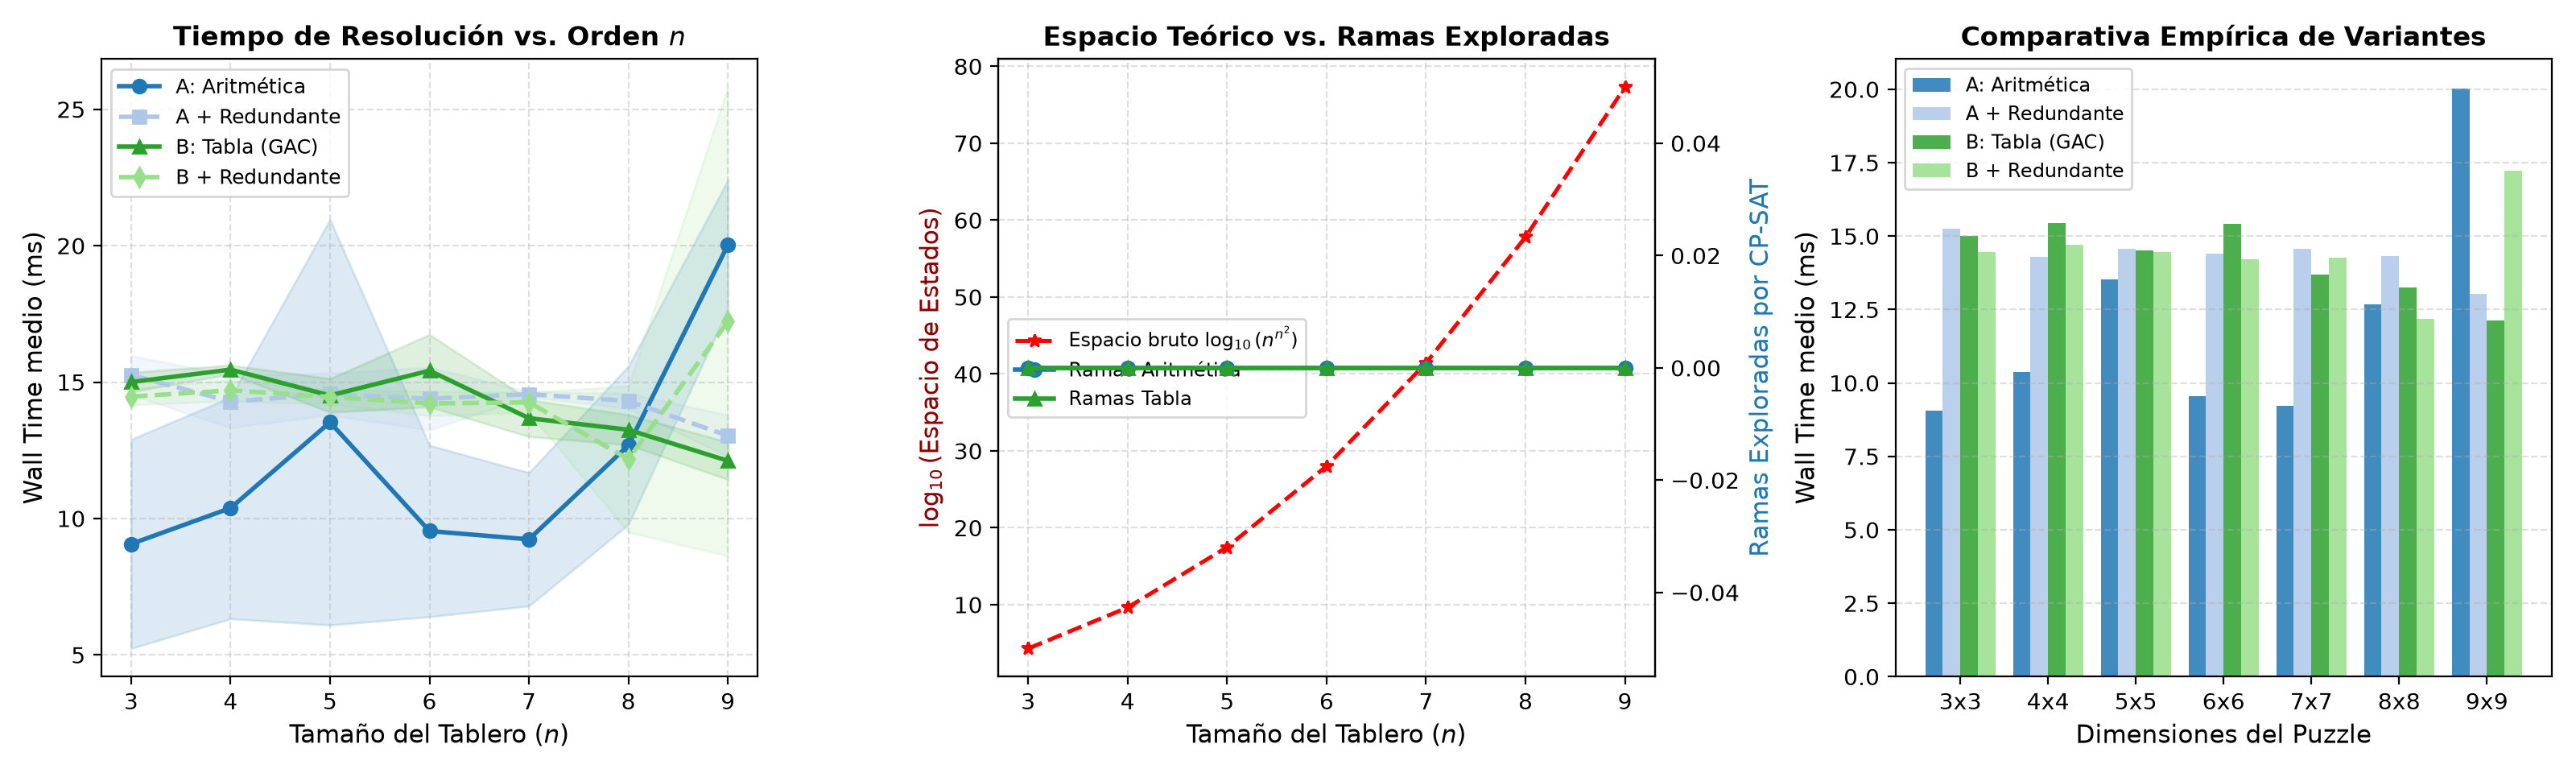
\includegraphics[width=\linewidth]{figs/cp_benchmark.png}
\caption{Evaluaci\'on emp\'{\i}rica del solver CP-SAT ($n=3$ a $9$): (a) Tiempo de ejecuci\'on medio por variante de modelado, (b) Crecimiento exponencial del espacio de estados bruto en escala logar\'{\i}tmica, (c) Ramas exploradas y conflictos reportados por el solver.}
\label{fig:cp_benchmark}
\end{figure}

\subsection{Discusi\'on de Hallazgos Emp\'{\i}ricos}
A partir de la evidencia experimental se verifican tres conclusiones fundamentales:

\begin{enumerate}
    \item \textbf{Eficacia del Filtrado GAC en Gran Escala (Variante B):} Para \'ordenes reducidos ($n \le 6$), el tiempo de construcci\'on y compilaci\'on de las tablas de tuplas introduce una ligera sobrecarga ($\approx 15\text{ ms}$). No obstante, en la m\'axima dimensi\'on evaluada ($n=9$), la Variante B extensional resolvi\'o el problema en \textbf{12.11 ms}, superando a la Variante A intensional (20.03 ms), lo que representa una \textbf{aceleraci\'on neta del 39.5\%}. El mantenimiento de Consistencia de Arco Generalizada poda combinaciones espurias antes de iniciar la propagaci\'on booleana.
    \item \textbf{Efecto Dual de las Restricciones Redundantes:} Para tableros peque\~nos ($n \le 6$), incorporar la suma Gaussiana (\ref{eq:redundant_sum}) incrementa el tiempo de resoluci\'on en $4$--$5\text{ ms}$ debido al coste de propagaci\'on de restricciones lineales redundantes. Sin embargo, para $n=9$, la restricci\'on redundante acelera la Variante A en un $35\%$ ($20.03\text{ ms} \to 13.03\text{ ms}$), confirmando que las restricciones implicadas resultan ventajosas cuando la combinatoria del problema explota.
    \item \textbf{Resoluci\'on en Nodo Ra\'{\i}z con Cero Backtracking:} En todas las dimensiones evaluadas ($n \in [3, 9]$) y en todas las variantes de modelado, el solver report\'o exactamente \textbf{0 ramas} y \textbf{0 conflictos}. Esto demuestra que la propagaci\'on acoplada de restricciones globales de Cuadrado Latino y las restricciones de jaula es lo suficientemente restrictiva como para resolver KenKen deterministamente sin incurrir en b\'usqueda combinatoria profunda.
\end{enumerate}
